\section{Declarative Knowledge Graph Construction}
\label{sec:chp2_declarative_kgc}

\ana{overview de distintas formas y métodos en general de construir KGs. Debería ser algo larga, ampliando lo que hay en la intro. Luego terminar con enfocarse en los approaches declarativos, que se extienden en la siguiente subsección}

%\ana{RAW} In this section, the current scene of mapping languages is described first, regardless of the approach they follow, i.e., RDF materialization or virtualization. Then, previous works comparing mapping languages are surveyed. 



\subsection{Declarative Mapping Rules}

\ana{DEFINICIÓN (mejor no poner como tal subsección y describir tal cual?)}

\ana{Empezar por qué es un mapping, quizá hablar de los otros tipos, y terminar escogiendo la definición que se aplica a los mappings d elos que se va a hablar el resto de la tesis, de datos (semi)estructurados a RDF. Intentar hacer algo de formalización ya de paso, aunque solo sea para esta parte de definir. }

\ana{pero es que igual cuadra más en el SOTA, porque como tal no estoy proponiendo una definición, sino cogiendo de otras ya hechas. }

\ana{Por ahora la que más cuadra es la sección 2 del paper-review de DylanVA. "Data Integration: A Theoretical Perspective" va encaminado, pero luego se mete en muchisimo detalle.}


Following, we present an overview of existing mapping languages, listed in \cref{tab:chp2_languages_summary}. We classify these languages in three categories depending on the schema they are based on or extend: RDF-based, SPARQL-based, and based on other schemas. An overview of the evolution, extensions and influences of these languages is depicted in \cref{fig:chp2_mapping_languages}.



\begin{figure*}[h]
\centering
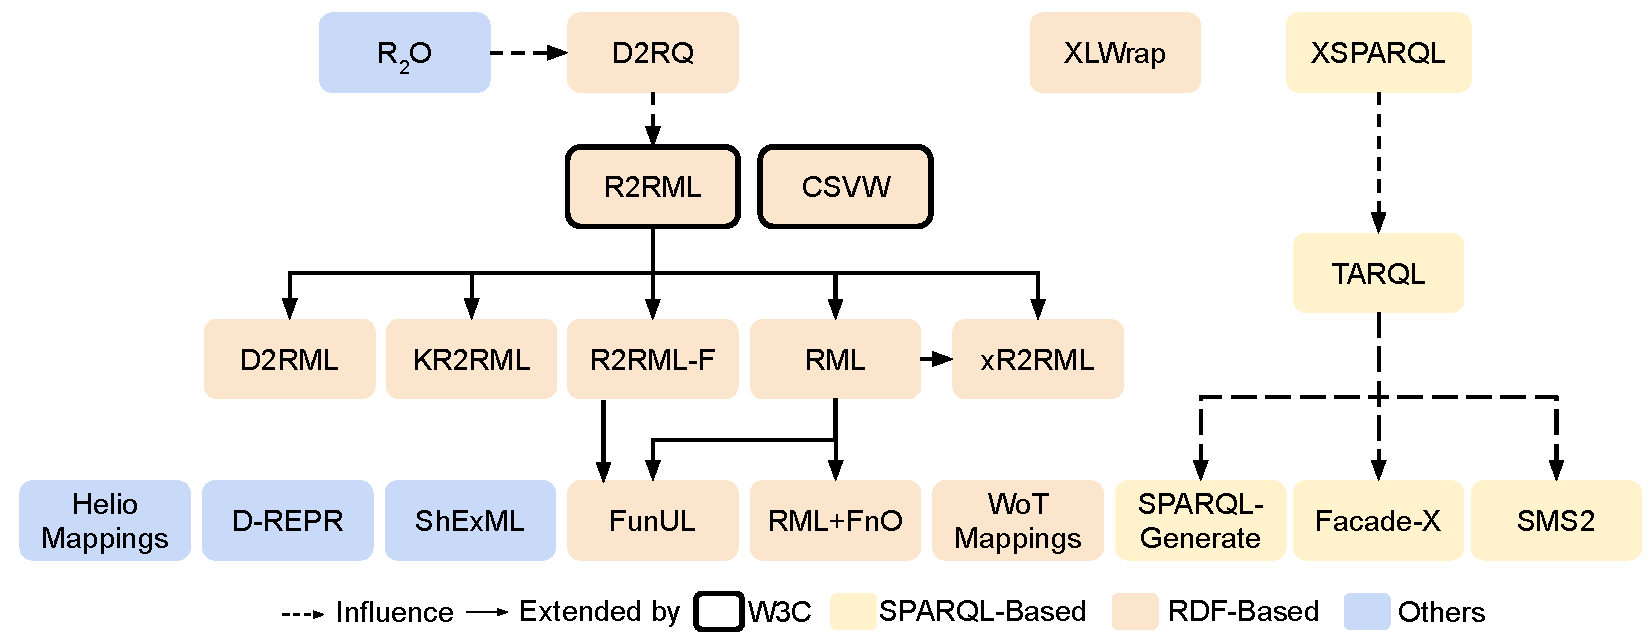
\includegraphics[width=0.95\linewidth]{figures/chp2_mapping_languages}
\caption[Existing mapping languages and the relationships among them]{Existing mapping languages and the relationships among them.}
\label{fig:chp2_mapping_languages}
\end{figure*}

\begin{table}[t]
\caption[Mapping languages overview]{Analyzed mapping languages and their corresponding references. \ana{pensar en eliminar helio, la versión nueva igual no entra dentro de esto y puede que cuadre quitar SMS2 y ponerlo luego con el análisis de las sintaxis}}
\label{tab:chp2_languages_summary}
\begin{tabular}{c|c|c}
\hline
%\rowcolor[HTML]{EFEFEF} 
Classification                 & Language        & Reference(s) \\ \hline
\multirow{11}{*}{RDF-based}   & D2RQ            & \parencite{bizer2004d2rq,d2rq}\\ \cline{2-3} 
                              & R$_2$O          & \parencite{barrasa2004r2o}\\ \cline{2-3} 
                              & R2RML           & \parencite{das2012r2rml}\\ \cline{2-3} 
                              & xR2RML          & \parencite{michel2015xr2rml,xr2rml}\\ \cline{2-3} 
                              & RML             & \parencite{Dimou2014rml,rml}\\ \cline{2-3} 
                              & KR2RML          & \parencite{slepicka2015kr2rml}\\ \cline{2-3} 
                              & FunUL           & \parencite{junior2016funul}\\ \cline{2-3} 
                              & R2RML-f         & \parencite{debruyne2016r2rmlf}\\ \cline{2-3} 
                              & D2RML           & \parencite{chortaras2018d2rml}\\ \cline{2-3}  
                              & WoT mappings    & \parencite{cimmino2020ewot}\\ \cline{2-3} 
                              & XLWrap          & \parencite{langegger2009xlwrap,xlwrap}\\ \cline{2-3} 
                              & CSVW            & \parencite{Tennison2015csvw}\\ \hline
\multirow{4}{*}{SPARQL-based} & SPARQL-Generate &     
                              \parencite{Lefrancois2017sparqlgenerate,sparqlgenerate}\\ \cline{2-3} 
                              & XSPARQL         & \parencite{Bischof2012xsparql,xsparql}\\ \cline{2-3} 
                              & TARQL           & \parencite{tarql}\\ \cline{2-3}
                              & Facade-X        & \parencite{asprino2023sparql-anything,sparqlanything}\\ \cline{2-3}
                              & SMS2            & \parencite{sms2}\\ \hline
\multirow{3}{*}{Others}       & Helio mappings  & \parencite{cimmino2022helio}\\ \cline{2-3} 
                              & D-REPR          & \parencite{Vu2019d-repr}\\ \cline{2-3} 
                              & ShExML          & \parencite{Garcia-Gonzalez2020shexml,shexml}\\ \cline{2-3}
                              & XRM             & \parencite{xrm}\\ \hline
\end{tabular}
\end{table}

\subsubsection{RDF-based mapping languages.} 

This group of languages are specified as ontologies or vocabularies able to describe the transformation rules of heterogeneous data into RDF. They are written in RDF documents, usually using the Turtle syntax~\parencite{turtle}. 



\noindent\textbf{D2RQ}~\parencite{bizer2004d2rq}

\noindent\textbf{XLWrap}~\parencite{langegger2009xlwrap}

\noindent\textbf{R2RML}~\parencite{das2012r2rml}

\noindent\textbf{R2RML-f}~\parencite{debruyne2016r2rmlf}

\noindent\textbf{RML}~\parencite{Dimou2014rml}

\noindent\textbf{FunUL}~\parencite{junior2016funul}

\noindent\textbf{KR2RML}~\parencite{slepicka2015kr2rml}

\noindent\textbf{xR2RML}~\parencite{michel2015xr2rml}

\noindent\textbf{D2RML}~\parencite{chortaras2018d2rml}

\noindent\textbf{CSVW}~\parencite{Tennison2015csvw}

\noindent\textbf{WoT Mappings}~\parencite{cimmino2020ewot}

\textit{The most well-known language in this category is R2RML~\parencite{das2012r2rml}, which allows mapping of data stored in relational databases to RDF. This language is heavily influenced by previous languages (R$_2$O~\parencite{barrasa2004r2o} and D2RQ~\parencite{bizer2004d2rq}). Some serializations (e.g. SML~\parencite{Stadler2015sml}, OBDA mappings from Ontop~\parencite{rodriguez2015efficient}) and several extensions of R2RML were developed in the following years after its release: R2RML-f~\parencite{debruyne2016r2rmlf} extends R2RML to include functions to be applied over the data; RML~\parencite{Dimou2014rml} and its user-friendly compact syntax YARRRML~\parencite{Heyvaert2018yarrrml} provide the possibility of covering additional data formats (CSV, XML and JSON); this language also considers the use of functions for data transformation (e.g. lowercase, replace, trim) by using the Function Ontology (FnO)\footnote{\url{https://fno.io/rml/}}~\parencite{DeMeester2017fno_dbpedia}; FunUL~\parencite{junior2016funul} proposes an extension to also incorporate functions, but focusing on the CSV format; KR2RML~\parencite{slepicka2015kr2rml} is also an extension for CSV, XML and JSON, with the addition of representing all sources with the Nested Relational Model as an intermediate model and the possibility of cleaning data with Python functions; xR2RML~\parencite{michel2015xr2rml} extends R2RML and RML to include NoSQL databases and incorporates more features to handle tree-like data; D2RML~\parencite{chortaras2018d2rml}, also based on R2RML and RML, is able to transform data from XML, JSON, CSVs and REST/SPARQL endpoints, and enables functions and conditions to create triples. }

\textit{In this category, we can also find more languages not related to R2RML. XLWrap~\parencite{langegger2009xlwrap} is focused on transforming spreadsheets into different formats. CSVW~\parencite{Tennison2015csvw} enables tabular data annotation on the Web with metadata, but also supports the generation of RDF. Finally, WoT Mappings~\parencite{cimmino2020ewot} are oriented to be used in the context of the Web of Things.}




\subsubsection{SPARQL-based mapping languages.} 

This group is integrated by languages that leverage the SPARQL query language, usually by extending its features to describe non-RDF data sources~\parencite{harris2013sparql}. 


\noindent\textbf{XSPARQL}~\parencite{Bischof2012xsparql}

\noindent\textbf{TARQL}~\parencite{tarql}

\noindent\textbf{SPARQL-Generate}~\parencite{Lefrancois2017sparqlgenerate}

\noindent\textbf{SPARQL-Anything}~\parencite{asprino2023sparql-anything}

\noindent\textbf{Sansa/whatever}~\parencite{stadler2023spark}




\textit{XSPARQL~\parencite{Bischof2012xsparql} merges SPARQL and XQuery to transform XML into RDF. TARQL~\parencite{tarql} uses the SPARQL syntax to generate RDF from CSV files. SPARQL-Generate~\parencite{Lefrancois2017sparqlgenerate} is capable of generating RDF and document streams from a wide variety of data formats and access protocols. Most recently, Facade-X has been developed, not as a new language, but as a "\textit{facade} to wrap the original resource and to make it queryable as if it was RDF"~\parencite{asprino2023sparql-anything}. It does not extend the SPARQL language, instead it overrides the SERVICE operator. Lastly, authors would like to highlight a loosely SPARQL-based language, Stardog Mapping Syntax 2 (SMS2)~\parencite{sms2}, which represents virtual Stardog graphs and is able to support sources such as JSON, CSV, RDB, MongoDB and Elasticsearch.}




\subsubsection{Based on other schemas.} 

Lastly, the languages of this group rely on schemas different from RDF or SPARQL, equally able and expressive enough to enable users to write transformation rules. 


\noindent\textbf{R$_2$O}~\parencite{barrasa2004r2o} XML-based~\footnote{https://pdfs.semanticscholar.org/4c47/0826aafc07fc6d37ca7e2474c1d3b290ade1.pdf}

\noindent\textbf{ShExML}~\parencite{Garcia-Gonzalez2020shexml,garcia2021shexml-challenges}

\noindent\textbf{Helio??}~\parencite{cimmino2022helio}

\noindent\textbf{D-REPR}~\parencite{Vu2019d-repr}

\textit{ShExML~\parencite{Garcia-Gonzalez2020shexml,garcia2021shexml-challenges} uses Shape Expressions (ShEx)~\parencite{prud2014shex} to map data sources in RDBs, CSV, JSON, XML and RDF using SPARQL queries. The Helio mapping language~\parencite{cimmino2022helio} is based on JSON and provides the capability of using functions for data transformation and data linking~\parencite{cimmino2018hybrid}. D-REPR~\parencite{Vu2019d-repr} focuses on describing heterogeneous data with JSONPath and allows the use of data transformation functions. XRM (Expressive RDF Mapper)~\parencite{xrm} is a commercial language that provides a unique user-friendly syntax to create mappings in R2RML, CSVW and RML.}










\subsection{Mapping Languages Comparison}
As the number of mapping languages increased and their adoption grew wider, comparisons between these languages inevitably occurred. This is the case of, for instance, SPARQL-Generate~\parencite{Lefrancois2017sparqlgenerate}, which is compared to RML in terms of query/mapping complexity; and ShExML~\parencite{Garcia-Gonzalez2020shexml}, which is compared to SPARQL-Generate and YARRRML from a usability perspective.

Some studies dig deeper, providing qualitative complex comparison frameworks. Hert et al.~\parencite{hert2011comparison} provide a comparison framework for mapping languages focused on transforming relational databases to RDF. The framework is composed of 15 features, and the languages are evaluated based on the presence or absence of these features.% (Logical table to class, M:N relationships, project attributes, select conditions, user-defined instance URIs, literal to URIs, vocabulary reuse, transformation functions, datatypes, named graphs, blank nodes, integrity constraints, static metadata, one table to \textit{n} classes, and write support). 
The results lead authors to divide the mappings into four categories (direct mapping, read-only general-purpose mapping, read-write general-purpose mapping, and special-purpose mapping), and ponder on the heavy reliance of most languages on SQL to implement the mapping, and the usefulness of read-write mappings (i.e., mappings able to write data in the database). De Meester et al.~\parencite{DeMeester2019comparison} show an initial analysis of 5 similar languages (RML+FnO, xR2RML, FunUL, SPARQL-Generate, YARRRML) discussing their characteristics, according to three categories: non-functional, functional and data source support. The study concludes by remarking on the need to build a more complete and precise comparative framework and asking for a more active participation from the community to build it. To the best of our knowledge, there is no comprehensive work in the literature comparing all existing languages. \ana{ojo con esto que con el survey de ghent ya no es del todo cierto :(} 
